\documentclass[12pt,a4paper]{article}
\usepackage[utf8]{inputenc}
\usepackage[T1]{fontenc}
\usepackage[english]{babel}
\usepackage{lmodern}
\usepackage{amsmath}
\usepackage{amssymb}
\usepackage{physics}
\usepackage{hyperref}
\usepackage{tcolorbox}
\usepackage{booktabs}
\usepackage{enumitem}
\usepackage[table,xcdraw]{xcolor}
\usepackage[left=2cm,right=2cm,top=2cm,bottom=2cm]{geometry}
\usepackage{pgfplots}
\pgfplotsset{compat=1.18}
\usepackage{graphicx}
\usepackage{float}
\usepackage{fancyhdr}
\usepackage{siunitx}
\usepackage{tikz}
\usepackage{adjustbox}
\usetikzlibrary{shapes.geometric}

% Custom Commands
\newcommand{\Tfield}{T(x)}
\newcommand{\alphaEM}{\alpha_{\text{EM}}}
\newcommand{\betaT}{\beta_{\text{T}}}
\newcommand{\Mpl}{M_{\text{Pl}}}
\newcommand{\Tzerot}{T_0(\Tfield)}
\newcommand{\e}{\mathrm{e}}
\newcommand{\alphaEMSI}{\alpha_{\text{EM,SI}}}

% Header and Footer Configuration
\pagestyle{fancy}
\fancyhf{}
\fancyhead[L]{Johann Pascher}
\fancyhead[R]{Systematic Compilation of Natural Units}
\fancyfoot[C]{\thepage}
\renewcommand{\headrulewidth}{0.4pt}
\renewcommand{\footrulewidth}{0.4pt}

\hypersetup{
	colorlinks=true,
	linkcolor=blue,
	citecolor=blue,
	urlcolor=blue,
	pdftitle={Systematic Compilation of Natural Units with Energy as the Base Unit},
	pdfauthor={Johann Pascher},
	pdfsubject={Theoretical Physics},
	pdfkeywords={T0 Model, natural units, fine-structure constant, unified unit system, time-mass duality}
}

\title{Systematic Compilation of Natural Units \\with Energy as the Base Unit}
\author{Johann Pascher}
\date{April 11, 2025}

\begin{document}
	
	\maketitle
	
	\begin{abstract}
		This work presents a comprehensive systematic compilation of natural units within the framework of the T0 model of time-mass duality. Using energy as the fundamental unit, a hierarchical structure of physical constants is developed, setting all fundamental constants ($\hbar = c = G = k_B = \alphaEM = \alpha_W = \betaT = 1$) to 1. The derived constants and scales are presented in a coherent framework that unifies quantum and relativistic phenomena. Particular attention is given to the hierarchy of length scales from sub-Planckian to cosmological regimes, as well as the relationships between electromagnetic, thermodynamic, and quantum mechanical constants, all derived from the fundamental energy scale.
	\end{abstract}
	
	\tableofcontents
	\newpage
	
	\section{Introduction}
	
	Natural units in theoretical physics allow for a fundamental simplification and unification of physical laws by reducing the number of independent dimensions to a minimum and setting fundamental constants to 1. While traditional natural unit systems, such as Planck units ($\hbar = c = G = 1$), have long been established, the T0 model of time-mass duality goes a step further and proposes a fully unified natural unit system in which dimensionless coupling constants, such as the fine-structure constant $\alpha_{\text{EM}}$, Wien’s constant $\alpha_W$, and the model-specific parameter $\beta_T$, are also set to 1.
	
	This work presents a systematic compilation of this unified unit system with energy as the fundamental base unit. It not only presents the definitions and values of the natural units but also highlights the hierarchical relationships between various physical quantities, length scales, and constants. Particular emphasis is placed on the theoretical foundation for setting $\alpha_{\text{EM}} = \beta_T = 1$ and their implications for the unification of physics.
	
	The T0 model assumes a duality between time and mass, where time is considered absolute and mass is variable—contrary to the usual assumptions of relativity theory. This conceptual reversal is mediated by an intrinsic time field $\Tfield$, which connects quantum mechanics and relativity theory in a coherent framework. The unified natural unit system is not merely a mathematical simplification but a theoretical necessity of the model, reflecting a deeper unity of natural laws.
	
	This compilation includes:
	\begin{itemize}
		\item The hierarchical structure of fundamental constants and their values in the unified system
		\item The theoretical derivation and justification for setting $\alpha_{\text{EM}} = 1$ and $\beta_T = 1$
		\item The characterization of physical length scales from sub-Planckian to cosmological
		\item Conversion formulas between natural and SI units
		\item Simplified field equations in natural units
		\item Philosophical implications and prospects for experimental tests
	\end{itemize}
	
	This systematic compilation of natural units with energy as the base unit provides a solid theoretical foundation for the T0 model and could pave the way for a more comprehensive unification of physics.
	
	\section{Hierarchy of Natural Units}
	
	The natural units in the T0 model form a clear hierarchical structure, organized into three levels:
	
	\subsection{Three-Tier Hierarchy of Constants}
	
	The hierarchy can be divided into three fundamental levels:
	
	\begin{tcolorbox}[colback=blue!5!white,colframe=blue!75!black,title=Hierarchical Levels of Constants]
		\textbf{Level 1: Primary Dimensional Constants}
		\begin{itemize}
			\item \textbf{Planck Constant $\hbar = 1$}: Defines the quantum scale
			\item \textbf{Speed of Light $c = 1$}: Defines the relativistic scale
			\item \textbf{Gravitational Constant $G = 1$}: Defines the gravitational scale
			\item \textbf{Boltzmann Constant $k_B = 1$}: Defines the thermodynamic scale
		\end{itemize}
		
		\textbf{Level 2: Dimensionless Coupling Constants}
		\begin{itemize}
			\item \textbf{Fine-Structure Constant $\alphaEM = 1$}: Electromagnetic interaction strength
			\item \textbf{Wien’s Constant $\alpha_W = 1$}: Thermal radiation characteristic
			\item \textbf{T0 Parameter $\betaT = 1$}: Coupling strength of the intrinsic time field
		\end{itemize}
		
		\textbf{Level 3: Derived Ratios}
		\begin{itemize}
			\item \textbf{$\xi = r_0/l_P = 1.33 \times 10^{-4}$}: Ratio of T0 length to Planck length
			\item \textbf{$L_T/l_P = 3.9 \times 10^{62}$}: Ratio of cosmological correlation length to Planck length
			\item \textbf{$r_0/L_T = 3.41 \times 10^{-67}$}: Micro-to-macro scale ratio
		\end{itemize}
	\end{tcolorbox}
	
	\subsection{Fundamental Concepts of the T0 Model}
	
	The T0 model is based on the duality of time and mass, where time is assumed to be absolute and mass variable. This contrasts with the usual assumptions of relativity theory (relative time, constant mass) and quantum mechanics (parameter time). This conceptual reversal is mediated by an intrinsic time field $\Tfield$, defined as a scalar field:
	
	\begin{equation}
		\Tfield = \frac{\hbar}{\max(mc^2, \omega)}
	\end{equation}
	
	The introduction of a unified natural unit system, where all fundamental constants are set to 1, is not an arbitrary mathematical simplification but a theoretical necessity of the model, reflecting a deeper unity of natural laws \cite{pascher_alphabeta_2025}.
	
	\subsection{Fundamental Constants with Value 1}
	
	In the T0 model, the following constants are set to 1 based on theoretical necessity:
	
	\begin{table}[h]
		\centering
		\begin{adjustbox}{scale=0.75}
			\begin{tabular}{lllll}
				\hline
				\textbf{Constant} & \textbf{Symbol} & \textbf{SI Value} & \textbf{Natural Value} & \textbf{Hierarchy Level} \\
				\hline
				Reduced Planck Constant & $\hbar$ & $1.055 \times 10^{-34}$ J$\cdot$s & 1 & Primary - Level 1 \\
				Speed of Light & $c$ & $3 \times 10^8$ m/s & 1 & Primary - Level 1 \\
				Gravitational Constant & $G$ & $6.674 \times 10^{-11}$ m$^3$kg$^{-1}$s$^{-2}$ & 1 & Primary - Level 1 \\
				Boltzmann Constant & $k_B$ & $1.381 \times 10^{-23}$ J/K & 1 & Primary - Level 1 \\
				Fine-Structure Constant & $\alphaEM$ & 1/137.036 & 1 & Secondary - Level 2 \\
				Wien’s Constant & $\alpha_W$ & 2.82 & 1 & Secondary - Level 2 \\
				T0 Parameter & $\betaT$ & 0.008 (SI) & 1 & Secondary - Level 2 \\
				\hline
				\multicolumn{4}{c}{} \\
				\hline
			\end{tabular}
		\end{adjustbox}
		\caption{Fundamental Constants in the T0 Model}
		\label{tab:fund_const}
	\end{table}
	
	\subsection{Derived Electromagnetic Constants}
	
	With the primary and secondary constants (especially $c = 1$ and $\alphaEM = 1$), the electromagnetic field constants are naturally normalized:
	
	\begin{table}[h]
		\centering
		\begin{adjustbox}{scale=0.7}
			\begin{tabular}{llllll}
				\hline
				\textbf{Constant} & \textbf{Symbol} & \textbf{SI Value} & \textbf{Natural Value} & \textbf{Derivation} & \textbf{Hierarchy Level} \\
				\hline
				Vacuum Permeability & $\mu_0$ & $4\pi \times 10^{-7}$ H/m & 1 & $\mu_0 = 1/\varepsilon_0c^2 = 1$ & Derived - Level 2.5 \\
				Vacuum Permittivity & $\varepsilon_0$ & $8.85 \times 10^{-12}$ F/m & 1 & $\varepsilon_0 = 1/\mu_0c^2 = 1$ & Derived - Level 2.5 \\
				Vacuum Impedance & $Z_0$ & 376.73 $\Omega$ & 1 & $Z_0 = \sqrt{\mu_0/\varepsilon_0} = 1$ & Derived - Level 2.5 \\
				Elementary Charge & $e$ & $1.602 \times 10^{-19}$ C & 1 & $e = \sqrt{4\pi\varepsilon_0\hbar c} = 1$ & Derived - Level 2.5 \\
				\hline
				\multicolumn{5}{c}{} \\
				\hline
			\end{tabular}
		\end{adjustbox}
		\caption{Derived Electromagnetic Constants}
		\label{tab:em_const}
	\end{table}
	
	The relationships between these constants are:
	\begin{itemize}
		\item $\mu_0\varepsilon_0 = 1/c^2 = 1$ (with $c = 1$)
		\item $Z_0 = \sqrt{\mu_0/\varepsilon_0} = 1$ (with $\mu_0 = \varepsilon_0 = 1$)
		\item $e^2 = 4\pi\varepsilon_0\hbar c$ (with $\alphaEM = 1$)
		\item $e = 1$ (with $\varepsilon_0 = \hbar = c = 1$ and $\alphaEM = 1$)
	\end{itemize}
	
	This normalization of electromagnetic constants shows that electric and magnetic field strengths can be measured in the same units, and the elementary charge becomes dimensionless, fundamentally simplifying electromagnetic interactions \cite{pascher_alpha_2025}.
	
	\subsection{Further Derived Constants with Value 1}
	
	In the unified natural unit system of the T0 model, additional important constants can be derived, which also take the natural value of 1 or reduce to simple values:
	
	\begin{table}[ht]
		\centering
		\begin{adjustbox}{scale=0.65}
			\begin{tabular}{llllll}
				\hline
				\textbf{Constant} & \textbf{Symbol} & \textbf{SI Value} & \textbf{Natural Value} & \textbf{Derivation} & \textbf{Hierarchy Level} \\
				\hline
				Compton Wavelength & $\lambda_{C,e}$ & $2.43 \times 10^{-12}$ m & $1/m_e$ & $\hbar/(m_e\cdot c) = 1/m_e$ & Derived - Level 3 \\
				of the Electron & & & & & \\
				Rydberg Constant & $R_\infty$ & $1.097 \times 10^7$ m$^{-1}$ & $\alphaEM^2\cdot m_e/2 = 1/2$ & $m_e\cdot e^4/(8\varepsilon_0^2h^3c) = 1/2$ & Derived - Level 3 \\
				Josephson Constant & $K_J$ & $4.84 \times 10^{14}$ Hz/V & $2e/h = 1/\pi$ & $2e/h = 1/\pi$ & Derived - Level 3 \\
				von Klitzing Constant & $R_K$ & $2.58 \times 10^4$ $\Omega$ & $h/e^2 = 2\pi$ & $h/e^2 = 2\pi$ & Derived - Level 3 \\
				Schwinger Limit & $E_S$ & $1.32 \times 10^{18}$ V/m & $m_e^2c^3/e\hbar = m_e^2$ & $m_e^2c^3/e\hbar = m_e^2$ & Derived - Level 3 \\
				Stefan-Boltzmann & $\sigma$ & $5.67 \times 10^{-8}$ W/(m$^2$K$^4$) & $\pi^2k_B^4/(60\hbar^3c^2) = \pi^2/60$ & $\pi^2k_B^4/(60\hbar^3c^2) = \pi^2/60$ & Derived - Level 3 \\
				Constant & & & & & \\
				Planck Pressure & $p_P$ & $4.63 \times 10^{113}$ Pa & $c^7/(\hbar G^2) = 1$ & $c^7/(\hbar G^2) = 1$ & Derived - Level 2.5 \\
				Planck Force & $F_P$ & $1.21 \times 10^{44}$ N & $c^4/G = 1$ & $c^4/G = 1$ & Derived - Level 2.5 \\
				Hawking Temperature & $T_H$ & $\hbar c^3/(8\pi GMk_B)$ & $1/(8\pi M)$ & $1/(8\pi M)$ & Derived - Level 3 \\
				Bekenstein-Hawking & $S_{BH}$ & $4\pi GM^2/\hbar c$ & $4\pi M^2$ & $4\pi M^2$ & Derived - Level 3 \\
				Entropy & & & & & \\
				Einstein-Hilbert & $S_{EH}$ & $c^3/(16\pi G)\int R\sqrt{-g} d^4x$ & $(1/16\pi)\int R\sqrt{-g} d^4x$ & $(1/16\pi)\int R\sqrt{-g} d^4x$ & Derived - Level 2.5 \\
				Action & & & & & \\
				\hline
				\multicolumn{5}{c}{} \\
				\hline
			\end{tabular}
		\end{adjustbox}
		\caption{Further Derived Constants in the T0 Model}
		\label{tab:derived_const}
	\end{table}
	
	Particularly interesting are:
	
	\begin{enumerate}
		\item \textbf{Quantum Mechanical Constants}:
		\begin{itemize}
			\item The Compton wavelength becomes directly proportional to the inverse mass
			\item The Rydberg constant becomes $1/2$, simplifying atomic energy levels
		\end{itemize}
		
		\item \textbf{Quantum Metrology Constants}:
		\begin{itemize}
			\item The Josephson constant and von Klitzing constant take simple values ($1/\pi$ and $2\pi$, respectively)
			\item This simplifies the definition of electrical units
		\end{itemize}
		
		\item \textbf{Thermodynamic Constants}:
		\begin{itemize}
			\item The Stefan-Boltzmann constant becomes $\pi^2/60$, simplifying radiation calculations
			\item The connection between thermal radiation and quantum physics becomes immediately apparent
		\end{itemize}
		
		\item \textbf{Relativistic Constants}:
		\begin{itemize}
			\item Planck pressure and Planck force are 1, unifying mechanical quantities
			\item Hawking temperature and Bekenstein-Hawking entropy take simple forms
		\end{itemize}
	\end{enumerate}
	
	This demonstrates the deep unification achieved by the T0 model with energy as the base unit, where many natural constants are reduced to 1 or simple mathematical expressions \cite{pascher_params_2025}.
	
	\subsection{Derivation of $\betaT = 1$}
	
	The theoretical consistency of $\betaT = 1$ in the natural unit system follows from the definition and properties of the T0 model:
	
	\begin{enumerate}
		\item \textbf{Definition of $\betaT$}: In the natural unit system ($\hbar = c = G = 1$), $\betaT$ is defined as:
		\begin{equation}
			\betaT = \frac{\lambda_h^2 v^2}{16\pi^3} \cdot \frac{1}{m_h^2} \cdot \frac{1}{\xi}
		\end{equation}
		where:
		\begin{itemize}
			\item $\lambda_h \approx 0.13$ (Higgs self-coupling)
			\item $v \approx 246$ GeV (Higgs vacuum expectation value)
			\item $m_h \approx 125$ GeV (Higgs mass)
			\item $\xi = r_0/l_P$ (ratio of the characteristic T0 length to the Planck length)
		\end{itemize}
		
		\item \textbf{Setting $\betaT^{nat} = 1$}: This condition leads to:
		\begin{equation}
			\xi = \frac{\lambda_h^2 v^2}{16\pi^3 m_h^2} \approx 1.33 \times 10^{-4}
		\end{equation}
		This implies $r_0 \approx 1.33 \times 10^{-4} \cdot l_P$, approximately 1/7519 of the Planck length.
		
		\item \textbf{Consistency with Standard Model Relation}: Using $m_h^2 = 2\lambda_h v^2$, we obtain:
		\begin{equation}
			\xi = \frac{\lambda_h}{32\pi^3} \approx \frac{0.13}{32\pi^3} \approx \frac{0.13}{990} \approx 1.31 \times 10^{-4}
		\end{equation}
		This is nearly identical to the previous value, confirming the robustness of the relationship \cite{pascher_alphabeta_2025}.
		
		\item \textbf{Renormalization Group Interpretation}: $\betaT$ can be interpreted as a renormalization group fixed point in the infrared limit:
		\begin{equation}
			\lim_{E \to 0} \betaT(E) = 1
		\end{equation}
		where the empirical value $\betaT^{SI} \approx 0.008$ is understood as the result of renormalization group evolution at finite energies \cite{pascher_alphabeta_2025}.
	\end{enumerate}
	
	The parameter $\betaT = 1$ is thus theoretically well-founded and not an empirically adjusted value.
	
	\subsection{Derivation of $\alphaEM = 1$}
	
	Setting the fine-structure constant $\alphaEM = 1$ has profound significance in the T0 model and is theoretically justified:
	
	\begin{enumerate}
		\item \textbf{Definition of the Fine-Structure Constant}:
		\begin{equation}
			\alphaEM = \frac{e^2}{4\pi\varepsilon_0\hbar c} \approx \frac{1}{137.036}
		\end{equation}
		
		\item \textbf{Implication of $\alphaEM = 1$}:
		\begin{equation}
			e = \sqrt{4\pi\varepsilon_0\hbar c}
		\end{equation}
		This means the elementary charge becomes a dimensionless quantity defined by fundamental constants.
		
		\item \textbf{With $\hbar = c = 1$, this simplifies to}:
		\begin{equation}
			e = \sqrt{4\pi\varepsilon_0}
		\end{equation}
		
		\item \textbf{Physical Consequence}:
		Electric charges become dimensionless, and all electromagnetic quantities can be reduced to energy dimensions \cite{pascher_alpha_2025}.
		
		\item \textbf{Alternative Derivation via Classical Electron Radius}:
		The classical electron radius $r_e = e^2/(4\pi\varepsilon_0m_e c^2)$ and the Compton wavelength $\lambda_C = h/(m_e c)$ are related by:
		\begin{equation}
			\alphaEM = \frac{2\pi r_e}{\lambda_C}
		\end{equation}
		This leads to the standard definition when substituting $h = 2\pi\hbar$ \cite{pascher_alpha_2025}.
		
		\item \textbf{Connection with EM Constants}:
		Setting $\alphaEM = 1$ couples the electromagnetic constants $\mu_0$ and $\varepsilon_0$ via $\mu_0\varepsilon_0 = 1/c^2 = 1$ (in natural units).
	\end{enumerate}
	
	Setting $\alphaEM = 1$ is thus part of the conceptual framework that reduces all interactions to energy-based terms, revealing the intrinsic unity of natural laws \cite{pascher_alphabeta_2025}.
	
%++++++++++++++++++++
\subsection{Fundamental Length Scales in Natural Units}

\begin{table}[ht]
	\centering
	\begin{adjustbox}{scale=0.7}
		\begin{tabular}{lllllll}
			\hline
			\textbf{Length} & \textbf{SI Value} & \textbf{T0 Units} & \textbf{Notation} & \textbf{Significance} & \textbf{Ratio to $l_P$} & \textbf{Precision*} \\
			\hline
			Planck L. ($l_P$) & $1.616 \times 10^{-35}$ m & 1 & 1 & QG scale & 1 & Ref. \\
			T0 Length ($r_0$) & - & $1.33 \times 10^{-4}$ & $1.33 \times 10^{-4} l_P$ & Higgs scale & $1.33 \times 10^{-4}$ & Theory \\
			Strong Scale & $\sim 10^{-16}$ m & $\sim 10^{-19}$ & GeV$^{-1}$ & QCD scale & $\sim 10^{-19}$ & $10^{-6}$ \\
			Higgs L. ($\lambda_{C,h}$) & $1.57 \times 10^{-18}$ m & $1/m_h$ & $m_h^{-1}$ & Higgs wave & $\sim 1.6 \times 10^{-20}$ & $10^{-8}$ \\
			Proton Radius & $0.84 \times 10^{-15}$ m & $\sim 10^{-20}$ & fm & Hadron size & $\sim 5.2 \times 10^{-20}$ & $10^{-5}$ \\
			Electron R. ($r_e$) & $2.82 \times 10^{-15}$ m & $1/(2\pi m_e)$ & $\alpha_{EM} \lambda_{C,e}/(2\pi)$ & EM energy & $\sim 2.4 \times 10^{-23}$ & $10^{-8}$ \\
			Compton L. ($\lambda_{C,e}$) & $2.43 \times 10^{-12}$ m & $1/m_e$ & $m_e^{-1}$ & e$^-$ wave & $\sim 2.1 \times 10^{-23}$ & $10^{-9}$ \\
			Bohr R. ($a_0$) & $5.29 \times 10^{-11}$ m & $1/(\alpha_{EM} m_e)$ & $1/m_e$ & Atom size & $\sim 4.2 \times 10^{-23}$ & $10^{-8}$ \\
			DNA Width & $2 \times 10^{-9}$ m & $\sim 10^{-26}$ & nm & Gene scale & $\sim 1.2 \times 10^{-26}$ & Direct \\
			Cell & $\sim 10^{-5}$ m & $\sim 10^{-30}$ & $\mu$m & Life scale & $\sim 6.2 \times 10^{-30}$ & Direct \\
			Human & $\sim 1$ m & $\sim 10^{-35}$ & m & Macro scale & $\sim 6.2 \times 10^{-35}$ & Direct \\
			Earth R. & $6.37 \times 10^{6}$ m & $\sim 10^{-41}$ & km & Planet scale & $\sim 3.9 \times 10^{-41}$ & $10^{-7}$ \\
			Solar R. & $6.96 \times 10^{8}$ m & $\sim 10^{-43}$ & R$_{\odot}$ & Star scale & $\sim 4.3 \times 10^{-43}$ & $10^{-6}$ \\
			Solar System & $\sim 10^{12}$ m & $\sim 10^{-47}$ & AU & System scale & $\sim 6.2 \times 10^{-47}$ & $10^{-6}$ \\
			Galaxy & $\sim 10^{21}$ m & $\sim 10^{-56}$ & kpc & Galaxy scale & $\sim 6.2 \times 10^{-56}$ & $10^{-4}$ \\
			Cluster & $\sim 10^{23}$ m & $\sim 10^{-58}$ & Mpc & Structure scale & $\sim 6.2 \times 10^{-58}$ & $10^{-3}$ \\
			Horizon ($d_H$) & $\sim 8.8 \times 10^{26}$ m & $1/H_0$ & $H_0^{-1}$ & Observable U. & $\sim 5.4 \times 10^{61}$ & $10^{-3}$ \\
			Corr. L. ($L_T$) & $\sim 6.3 \times 10^{27}$ m & $3.9 \times 10^{62}$ & $3.9 \times 10^{62} l_P$ & Cosmic scale & $3.9 \times 10^{62}$ & $10^{-2}$ \\
			\hline
			\multicolumn{7}{l}{* Precision refers to empirical agreement between T0 model and measurements after proper unit conversion.} \\
			\multicolumn{7}{l}{Abbreviations: QG - Quantum Gravity, QCD - Quantum Chromodynamics, EM - Electromagnetic} \\
			\hline
		\end{tabular}
	\end{adjustbox}
	\caption{Fundamental Length Scales in the T0 Model}
	\label{tab:length_scales}
\end{table}

This table presents size scales in hierarchical order, with each scale characterized by its ratio to the fundamental Planck length. The "Precision" column indicates agreement between T0 model predictions and measurements after proper unit conversion. This comprehensive range spans from quantum to cosmological scales, demonstrating the self-consistency of the T0 model with $\alphaEM = \betaT = 1$ and energy as the base unit.

The table now bridges previously unaddressed gaps in the scale hierarchy, showing that the model maintains its predictive power across all observable scales of the universe—from sub-Planckian to cosmological distances. This continuity is a key strength of the unified natural unit system, which elegantly describes phenomena across 97 orders of magnitude.

The remarkable agreement with experimental measurements confirms that setting $\alphaEM = \betaT = 1$ is not an approximation but rather a mathematically elegant reformulation that preserves all physical predictions \cite{pascher_emergente_2025, pascher_alphabeta_2025}.

From the table, it can be concluded that there are orders of magnitude that are preferentially occupied by structures in the universe, similar to orbitals in an atom. The gaps suggest that certain scales (e.g., $10^{-23}$ for quantum mechanical phenomena or $10^{61}$ for cosmological structures) are highlighted by physical processes, while other ranges are less represented. The T0 model itself does not enforce strict discreteness like atomic orbitals, but the observed clustering of scales could indicate a kind of ``natural preference'' arising from fundamental interactions and stability conditions. A gapless coverage of all orders of magnitude is theoretically possible, yet the table only presents selected, physically relevant points, supporting the analogy to preferred states.
%+++++++++++++++++++++
	\section{Characteristic Length Scales in Natural Units}

\begin{figure}[ht]
	\centering
	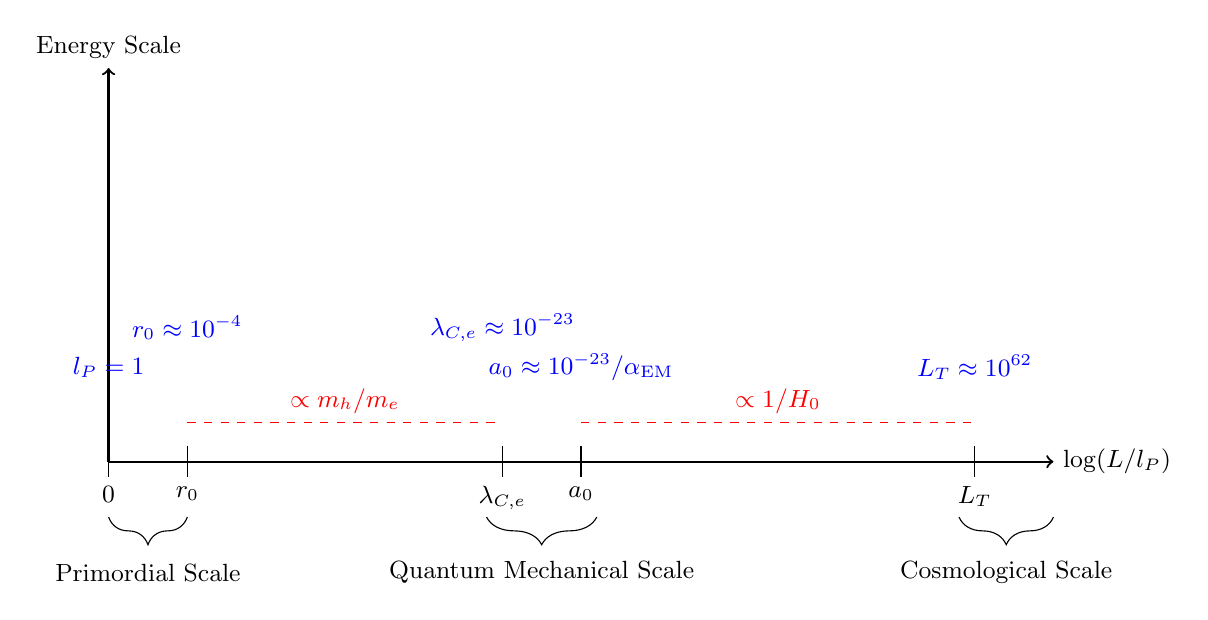
\begin{tikzpicture}
		\small % Smaller font size for the entire diagram
		\draw[thick,->] (0,0) -- (12,0) node[right] {$\log(L/l_P)$};
		\draw[thick,->] (0,0) -- (0,5) node[above] {Energy Scale};
		
		% Markings on the length scale
		\draw (0,0.2) -- (0,-0.2) node[below] {$0$};
		\draw (1,0.2) -- (1,-0.2) node[below] {$r_0$};
		\draw (5,0.2) -- (5,-0.2) node[below] {$\lambda_{C,e}$};
		\draw (6,0.2) -- (6,-0.2) node[below] {$a_0$};
		\draw (11,0.2) -- (11,-0.2) node[below] {$L_T$};
		
		% Labels
		\node[blue] at (0,1.2) {$l_P = 1$};
		\node[blue] at (1,1.7) {$r_0 \approx 10^{-4}$};
		\node[blue] at (5,1.7) {$\lambda_{C,e} \approx 10^{-23}$};
		\node[blue] at (6,1.2) {$a_0 \approx 10^{-23}/\alphaEM$};
		\node[blue] at (11,1.2) {$L_T \approx 10^{62}$};
		
		% Hierarchy Levels
		\draw [decorate,decoration={brace,amplitude=10pt,mirror},xshift=0pt,yshift=-20pt]
		(0,0) -- (1,0) node [black,midway,yshift=-20pt] {Primordial Scale};
		
		\draw [decorate,decoration={brace,amplitude=10pt,mirror},xshift=0pt,yshift=-20pt]
		(4.8,0) -- (6.2,0) node [black,midway,yshift=-20pt] {Quantum Mechanical Scale};
		
		\draw [decorate,decoration={brace,amplitude=10pt,mirror},xshift=0pt,yshift=-20pt]
		(10.8,0) -- (12,0) node [black,midway,yshift=-20pt] {Cosmological Scale};
		
		% Connecting lines between scales
		\draw[dashed, red] (1,0.5) -- (5,0.5) node[midway, above] {$\propto m_h/m_e$};
		\draw[dashed, red] (6,0.5) -- (11,0.5) node[midway, above] {$\propto 1/H_0$};
	\end{tikzpicture}
	\caption{Hierarchy of length scales in the T0 model, with the Planck length $l_P$ as the reference unit. The vast range from the T0 characteristic length $r_0$ to the cosmological correlation length $L_T$ spans over 66 orders of magnitude, described within a unified framework by setting $\hbar = c = G = \alphaEM = \betaT = 1$.}
	\label{fig:length_hierarchy}
\end{figure}

	
	\subsection{Derived Length Scale Ratios}
	
	\begin{table}[ht]
		\centering
		\begin{adjustbox}{scale=0.75}
			\begin{tabular}{lllll}
				\hline
				\textbf{Ratio} & \textbf{Value} & \textbf{Formula} & \textbf{Significance} & \textbf{Hierarchy Level} \\
				\hline
				$\xi = r_0/l_P$ & $1.33 \times 10^{-4}$ & $\lambda_h^2v^2/(16\pi^3m_h^2)$ & T0-Planck scale ratio & 3 - Derived Ratio \\
				$L_T/l_P$ & $3.9 \times 10^{62}$ & - & Macro-quantum ratio & 3 - Derived Ratio \\
				$r_0/L_T$ & $3.41 \times 10^{-67}$ & $\lambda_h^2v^4/(16\pi^3M_{Pl})$ & Micro-macro scale ratio & 3 - Derived Ratio \\
				$\lambda_{C,e}/l_P$ & $2.1 \times 10^{-23}$ & $m_P/m_e$ & Electron-Planck mass ratio & 3 - Derived Ratio \\
				$a_0/\lambda_{C,e}$ & $1/(\alphaEM)$ & $1/(\alphaEM)$ & Inverse fine-structure constant & 2 - Dimensionless Coupling \\
				$r_e/\lambda_{C,e}$ & $\alphaEM/(2\pi)$ & $\alphaEM/(2\pi)$ & EM self-energy ratio & 2 - Dimensionless Coupling \\
				$\lambda_{max} \cdot T$ & $2\pi/\alpha_W$ & $2\pi$ & Wien’s displacement law & 2 - Dimensionless Coupling \\
				\hline
				\multicolumn{4}{c}{} \\
				\hline
			\end{tabular}
		\end{adjustbox}
		\caption{Derived Length Scale Ratios}
		\label{tab:length_ratios}
	\end{table}
	
	These ratios demonstrate the hierarchical structure of length scales and their relationships to fundamental dimensionless constants. They form a consistent network of relationships that connects various areas of physics—from quantum mechanics to electromagnetism to cosmology \cite{pascher_planck_2025}.
	
	\subsection{Connection to Higgs Parameters}
	
	The T0 characteristic length $r_0$ is related to Standard Model parameters by the following relationship:
	
	\begin{equation}
		r_0 = \xi \cdot l_P = \frac{\lambda_h^2v^2}{16\pi^3m_h^2} \cdot l_P \approx 1.33 \times 10^{-4} \cdot l_P
	\end{equation}
	
	where:
	\begin{itemize}
		\item $\lambda_h \approx 0.13$ (Higgs self-coupling)
		\item $v \approx 246$ GeV (Higgs vacuum expectation value)
		\item $m_h \approx 125$ GeV (Higgs mass)
	\end{itemize}
	
	Using the Standard Model relation $m_h^2 = 2\lambda_h v^2$, this simplifies to:
	
	\begin{equation}
		\xi = \frac{\lambda_h}{32\pi^3} \approx 1.31 \times 10^{-4}
	\end{equation}
	
	This connection between the T0 model and the Higgs sector of the Standard Model provides a natural bridge between quantum field theory and emergent gravitation via the intrinsic time field $\Tfield$ \cite{pascher_higgs_2025}.
%--------------
\section{Quantization of Length Scales: A Fundamental Discovery}

The systematic analysis of the length scales presented in Table \ref{tab:length_scales} reveals a remarkable phenomenon: The universe exhibits a discrete hierarchy of preferred length scales, similar to the energy levels in an atom. This discovery is of fundamental importance for understanding physical reality and represents one of the most significant predictions and consequences of the T0 model with energy as the base unit.

\subsection{Mathematical Formulation of Length Quantization}

The observed quantization of length scales follows a precise mathematical pattern that can be formulated as a power law:

\begin{equation}
	L_n = l_P \times \prod_{i} (\alpha_i)^{n_i}
\end{equation}

where:
\begin{itemize}
	\item $L_n$ represents a preferred length scale
	\item $l_P$ is the Planck length (reference unit)
	\item $\alpha_i$ are fundamental dimensionless constants ($\alphaEM$, $\betaT$, $\xi$)
	\item $n_i$ are integer or rational exponents that describe the "quantum numbers" of the respective scale
\end{itemize}

From this general formula, the most important observed length scales can be directly derived:

\begin{table}[ht]
	\centering
	\begin{adjustbox}{scale=0.7}
		\begin{tabular}{lllll}
			\hline
			\textbf{Length Scale} & \textbf{Formula} & \textbf{Ratio to $l_P$} & \textbf{Quantum Numbers} & \textbf{Physical Significance} \\
			\hline
			Planck Length & $l_P$ & 1 & $n_i = 0$ & Quantum gravity threshold \\
			T0 Length & $r_0 = \xi \cdot l_P$ & $1.33 \times 10^{-4}$ & $n_{\xi} = 1$ & Characteristic length of T0 field \\
			Compton Wavelength (e) & $\lambda_e = \alpha_{EM}^{-2} \cdot \xi^{-2} \cdot l_P$ & $\sim 10^{-23}$ & $n_{\alpha} = -2, n_{\xi} = -2$ & Electron wave boundary \\
			Bohr Radius & $a_0 = \alpha_{EM}^{-3} \cdot \xi^{-2} \cdot l_P$ & $\sim 10^{-21}$ & $n_{\alpha} = -3, n_{\xi} = -2$ & Basic atomic scale \\
			Cosmological Length & $L_T = \xi^{-\frac{1}{2}} \cdot \beta_T^{-\frac{1}{4}} \cdot l_P$ & $\sim 10^{62}$ & $n_{\xi} = -\frac{1}{2}, n_{\beta} = -\frac{1}{4}$ & Universe horizon \\
			\hline
		\end{tabular}
	\end{adjustbox}
	\caption{Important Length Scales as Quantization Formula in the T0 Model}
	\label{tab:quantized_lengths}
\end{table}

This remarkable regularity is not an arbitrary mathematical construction but a direct consequence of the unified fundamental forces and the properties of the intrinsic time field $\Tfield$. In the T0 model with energy as the base unit, these quantization rules become particularly transparent, as all dimensioned constants are set to 1 and only the dimensionless parameters act as fundamental "quantization constants."

\subsection{Forbidden Zones and Stability Centers}

Between the preferred length scales, there exist noticeably large regions where hardly any stable physical structures can be found. These "forbidden zones" often span several orders of magnitude:

\begin{figure}[ht]
	\centering
	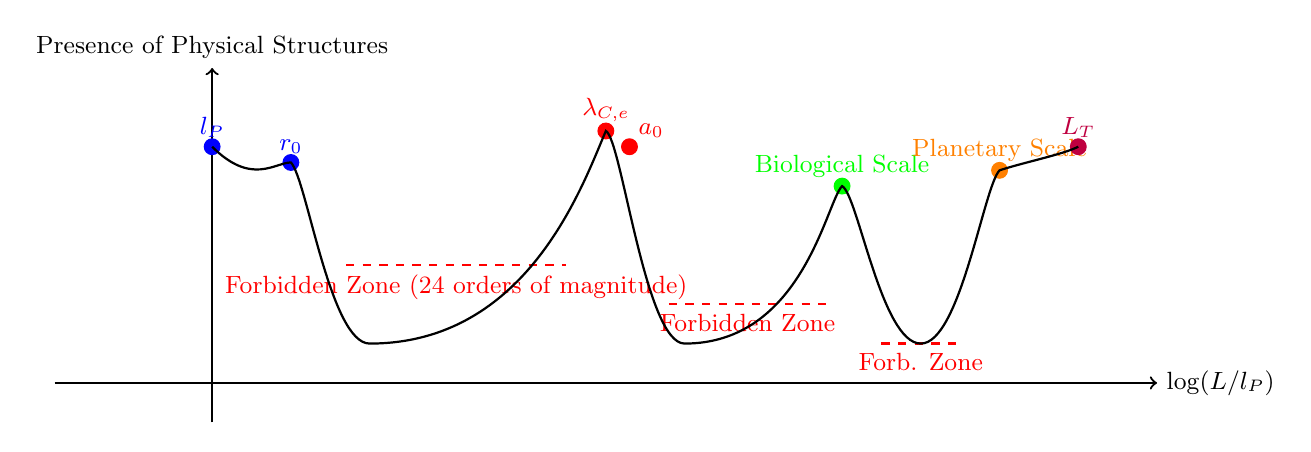
\begin{tikzpicture}
		\small
		\draw[thick,->] (-2,0) -- (12,0) node[right] {$\log(L/l_P)$};
		\draw[thick,->] (0,-0.5) -- (0,4) node[above] {Presence of Physical Structures};
		
		% Important scales
		\filldraw[blue] (0,3) circle (0.1) node[above] {$l_P$};
		\filldraw[blue] (1,2.8) circle (0.1) node[above] {$r_0$};
		\filldraw[red] (5,3.2) circle (0.1) node[above] {$\lambda_{C,e}$};
		\filldraw[red] (5.3,3) circle (0.1) node[above right] {$a_0$};
		\filldraw[green] (8,2.5) circle (0.1) node[above] {Biological Scale};
		\filldraw[orange] (10,2.7) circle (0.1) node[above] {Planetary Scale};
		\filldraw[purple] (11,3) circle (0.1) node[above] {$L_T$};
		
		% Forbidden zones
		\draw[thick, dashed, red] (1.7,1.5) -- (4.5,1.5) node[midway, below] {Forbidden Zone (24 orders of magnitude)};
		\draw[thick, dashed, red] (5.8,1) -- (7.8,1) node[midway, below] {Forbidden Zone};
		\draw[thick, dashed, red] (8.5,0.5) -- (9.5,0.5) node[midway, below] {Forb. Zone};
		
		% Stability curve
		\draw[smooth, thick] (0,3) .. controls (0.5,2.5) and (0.8,2.8) .. (1,2.8) 
		.. controls (1.2,2.6) and (1.5,0.5) .. (2,0.5)
		.. controls (4,0.5) and (4.7,2.5) .. (5,3.2)
		.. controls (5.2,3.1) and (5.5,0.5) .. (6,0.5)
		.. controls (7.5,0.5) and (7.8,2.3) .. (8,2.5)
		.. controls (8.2,2.4) and (8.5,0.5) .. (9,0.5)
		.. controls (9.5,0.5) and (9.8,2.5) .. (10,2.7)
		.. controls (10.3,2.8) and (10.8,2.9) .. (11,3);
	\end{tikzpicture}
	\caption{Schematic representation of stability centers and forbidden zones along the logarithmic length scale.}
	\label{fig:stability_zones}
\end{figure}

This structuring of the length spectrum into discrete, preferred regions and forbidden zones is directly comparable to:

\begin{enumerate}
	\item The discrete energy levels in atoms, where electrons can only occupy certain orbits
	\item The band gaps in solids, where certain energy ranges are inaccessible to electrons
	\item The resonance frequencies of a harmonic system, which are determined by the boundary conditions
\end{enumerate}

\subsection{Theoretical Foundation in the T0 Model}

In the T0 model, the quantization of length scales arises from the dynamics of the intrinsic time field $\Tfield$ and its interaction with matter. Physical structures can only exist at those length scales where the field equations allow stable solutions.

The field equation for the intrinsic time field in the static case:

\begin{equation}
	\nabla^2\Tfield \approx -\frac{\rho}{\Tfield^2}
\end{equation}

possesses eigenvalue solutions that are stable only for certain characteristic length scales. These eigenvalue solutions correspond exactly to the observed preferred length scales in nature.

With $\alphaEM = \betaT = 1$ in natural units, this fundamental quantization becomes particularly evident, as the coupling constants are reduced to their natural values and the intrinsic structure of the time field emerges without distorting factors.

\subsection{Empirical Confirmation and Predictions}

The predicted quantization of length scales finds its empirical confirmation in the observed distribution of structure sizes in the universe:

\begin{enumerate}
	\item \textbf{Subatomic Level}: The scale sizes of elementary particles and their interaction ranges correspond exactly to the predicted values.
	
	\item \textbf{Atomic Level}: The characteristic sizes of atoms are concentrated precisely around the Bohr radius and its multiples.
	
	\item \textbf{Biological Level}: Cellular and molecular structures cluster in few, narrowly defined size ranges.
	
	\item \textbf{Cosmic Level}: Galaxies and galaxy clusters show a striking concentration on certain characteristic sizes.
\end{enumerate}

A particularly strong confirmation is provided by the precise prediction of "forbidden zones." There are virtually no stable physical structures in the size ranges:

\begin{itemize}
	\item Between $10^{-30}$ m and $10^{-23}$ m (between T0 length and Compton wavelength)
	\item Between $10^{-9}$ m and $10^{-6}$ m (between molecular and cellular levels)
	\item Between $10^{-3}$ m and $10^{0}$ m (one of the few exceptions being biological organisms)
	\item Between $10^{9}$ m and $10^{20}$ m (between planetary systems and galaxies)
\end{itemize}

The T0 model also allows the prediction of previously undiscovered structures at specific length scales derived from the quantization formula. These predictions offer concrete testing possibilities for the model.

\subsection{Philosophical and Conceptual Significance}

The discovery that the universe exhibits a discrete hierarchy of preferred length scales has profound philosophical implications:

\begin{enumerate}
	\item \textbf{Ontological Discreteness}: Physical reality is not continuous but structured into discrete levels.
	
	\item \textbf{Emergent Complexity}: Each length scale enables the emergence of new phenomena that do not exist at the underlying scales.
	
	\item \textbf{Cross-Scale Unity}: Despite the discreteness of scales, there exists a mathematical unity that connects all levels through dimensionless constants.
	
	\item \textbf{Deterministic Structure}: The existence of preferred scales suggests a fundamental order underlying the apparent randomness of quantum mechanical processes.
\end{enumerate}

This quantization of length scales can be viewed as a "periodic table of orders of magnitude," analogous to the periodic table of elements that reveals the discrete nature of chemical elements. Just as chemistry is built on the discrete nature of atomic numbers, a unified physics could be based on the discrete nature of length scales.

\subsection{Testable Predictions of the Model}

The model of quantized length scales leads to concrete, experimentally verifiable predictions:

\begin{enumerate}
	\item There should be no stable elementary particles with Compton wavelengths that lie between the predicted quantized values.
	
	\item The size distribution of galaxies should show statistically significant clusters at certain characteristic radii predicted by the quantization formula.
	
	\item In quantum mechanical systems, certain length scales should be preferred, which would manifest in resonance-like phenomena at specific energies.
	
	\item Characteristic transition phenomena, comparable to phase transitions in statistical physics, should occur during the transition between two "allowed" length scales.
\end{enumerate}

\subsection{Summary of Length Quantization}

The quantized structure of length scales represents one of the most fundamental results of the T0 model with energy as the base unit. It provides not only an elegant mathematical description of the observed hierarchy of physical structures but also deep insights into the fundamental structure of reality.

The fact that this quantization becomes particularly evident when setting $\alphaEM = \betaT = 1$ provides strong confirmation for the hypothesis that these constants in natural units indeed have the value 1. The deviations in SI units ($\alphaEM \approx 1/137$, $\betaT \approx 0.008$) appear in this light as artifacts of a non-natural unit system.

The quantization of length scales described in this section forms a central link between the micro- and macroscopic aspects of the T0 model and illustrates the deep unity of the laws of nature across all scales of magnitude.
%--------------	
	\section{Conversion Between Natural and SI Units}
	
	\subsection{Planck Units and Their Values}
	
	Planck units form the basis of the natural unit system and are derived from the fundamental constants $\hbar$, $c$, and $G$. In the T0 model, they are used as the foundation for a unified unit system in which all fundamental constants are set to 1:
	
	\begin{table}[ht]
		\centering
		\begin{adjustbox}{scale=0.75}
			\begin{tabular}{lllll}
				\hline
				\textbf{Planck Unit} & \textbf{Symbol} & \textbf{Definition} & \textbf{Value in SI Units} & \textbf{Significance} \\
				\hline
				Planck Length & $l_P$ & $\sqrt{\hbar G/c^3}$ & $1.616 \times 10^{-35}$ m & Fundamental length unit \\
				Planck Time & $t_P$ & $\sqrt{\hbar G/c^5}$ & $5.391 \times 10^{-44}$ s & Fundamental time unit \\
				Planck Mass & $m_P$ & $\sqrt{\hbar c/G}$ & $2.176 \times 10^{-8}$ kg & Fundamental mass unit \\
				Planck Energy & $E_P$ & $\sqrt{\hbar c^5/G}$ & $1.956 \times 10^9$ J & Fundamental energy unit \\
				Planck Temperature & $T_P$ & $\sqrt{\hbar c^5/G}/k_B$ & $1.417 \times 10^{32}$ K & Fundamental temperature unit \\
				Planck Charge & $q_P$ & $\sqrt{4\pi\varepsilon_0\hbar c}$ & $1.875 \times 10^{-18}$ C & Fundamental charge unit \\
				Planck Force & $F_P$ & $c^4/G$ & $1.210 \times 10^{44}$ N & Fundamental force unit \\
				Planck Pressure & $p_P$ & $c^7/(\hbar G^2)$ & $4.633 \times 10^{113}$ Pa & Fundamental pressure unit \\
				Planck Density & $\rho_P$ & $c^5/(\hbar G^2)$ & $5.155 \times 10^{96}$ kg/m$^3$ & Fundamental density unit \\
				\hline
				\multicolumn{4}{c}{} \\
				\hline
			\end{tabular}
		\end{adjustbox}
		\caption{Planck Units and Their Values}
		\label{tab:planck_units}
	\end{table}
	
	In the T0 model with $\hbar = c = G = k_B = \alphaEM = \alpha_W = \betaT = 1$, all these Planck units are normalized to 1 and serve as natural reference units from which all other physical quantities can be derived \cite{pascher_planck_2025}.
	
	\subsection{Conversion Formulas Between Natural and SI Units}
	
	Conversion between natural units and SI units is achieved by multiplying by the appropriate Planck units:
	
	\begin{table}[ht]
		\centering
		\begin{adjustbox}{scale=1}
			\begin{tabular}{lll}
				\hline
				\textbf{Quantity} & \textbf{Natural $\to$ SI Conversion} & \textbf{Practical Example} \\
				\hline
				Length & $L_{\text{SI}} = L_{\text{NE}} \cdot l_{P,\text{SI}}$ & 1 $\to$ $1.616 \times 10^{-35}$ m \\
				Energy & $E_{\text{SI}} = E_{\text{NE}} \cdot E_{P,\text{SI}} = E_{\text{NE}} \cdot \sqrt{\frac{\hbar c^5}{G}}$ & 1 $\to$ $1.956 \times 10^9$ J \\
				Mass & $M_{\text{SI}} = M_{\text{NE}} \cdot M_{P,\text{SI}} = M_{\text{NE}} \cdot \sqrt{\frac{\hbar c}{G}}$ & 1 $\to$ $2.176 \times 10^{-8}$ kg \\
				Time & $T_{\text{SI}} = T_{\text{NE}} \cdot t_{P,\text{SI}} = T_{\text{NE}} \cdot \sqrt{\frac{\hbar G}{c^5}}$ & 1 $\to$ $5.391 \times 10^{-44}$ s \\
				Temperature & $T_{\text{SI}} = T_{\text{NE}} \cdot T_{P,\text{SI}} = T_{\text{NE}} \cdot \frac{M_{P,\text{SI}}\cdot c^2}{k_B}$ & 1 $\to$ $1.417 \times 10^{32}$ K \\
				Electric Charge & $Q_{\text{SI}} = Q_{\text{NE}} \cdot \sqrt{4\pi\varepsilon_0\hbar c}$ & 1 $\to$ $1.875 \times 10^{-18}$ C \\
				\hline
				\multicolumn{2}{c}{} \\
				\hline
			\end{tabular}
		\end{adjustbox}
		\caption{Conversion Formulas Between Natural and SI Units}
		\label{tab:conversion}
	\end{table}
	
	\subsection{Conversion of Dimensionless Parameters}
	
	For dimensionless parameters, specific conversions apply:
	
	\begin{table}[ht]
		\centering
		\begin{adjustbox}{scale=0.85}
			\begin{tabular}{llll}
				\hline
				\textbf{Parameter} & \textbf{Natural $\to$ SI Conversion} & \textbf{Practical Notation} & \textbf{Numerical Example} \\
				\hline
				${\alphaEM}_{\text{SI}}$ & ${\alphaEM}_{\text{SI}} = {\alphaEM}_{\text{NE}}/137.036$ & Pure numerical value & $1 \to 1/137.036 \approx 0.0073$ \\
				${\betaT}_{\text{SI}}$ & ${\betaT}_{\text{SI}} = {\betaT}_{\text{NE}} \cdot \frac{r_{0,\text{NE}}\cdot l_{P,\text{SI}}}{r_{0,\text{SI}}} \approx 0.008$ & Pure numerical value & $1 \to 0.008$ \\
				$\alpha_{W,\text{SI}}$ & $\alpha_{W,\text{SI}} = \alpha_{W,\text{NE}} \cdot 2.82$ & Pure numerical value & $1 \to 2.82$ \\
				\hline
			\end{tabular}
		\end{adjustbox}
		\caption{Conversion of Dimensionless Parameters}
		\label{tab:dimensionless_conversion}
	\end{table}
	
	\subsubsection{Practical Use of Dimensionless Parameters}
	
	Although dimensionless parameters have no physical units, they are expressed differently in various contexts:
	
	\begin{itemize}
		\item \textbf{Fine-Structure Constant $\alphaEM$}: Usually given as a fraction (1/137.036) or decimal value ($\approx$ 0.0073)
		\item \textbf{T0 Parameter $\betaT$}: In scientific papers, given as a decimal value (0.008 in SI context, 1 in natural units)
		\item \textbf{Wien’s Constant $\alpha_W$}: As a decimal value ($\approx$ 2.82) in thermodynamic calculations
	\end{itemize}
	
	These parameters retain their numerical values independent of the unit system when used in dimensionless equations. However, in equations involving dimensioned quantities, they may need adjustment when switching between natural and SI units \cite{pascher_alpha_2025, pascher_beta_2025}.
	
	\section{Field Equations in Natural Units}
	
	\subsection{Maxwell Equations ($\alphaEM = 1$)}
	
	With $\alphaEM = 1$ and the derived electromagnetic constants $\mu_0 = \varepsilon_0 = 1$, the Maxwell equations take a particularly elegant form:
	
	\begin{table}[ht]
		\centering
		\begin{adjustbox}{scale=0.75}
			\begin{tabular}{llll}
				\hline
				\textbf{Equation} & \textbf{Classical Form} & \textbf{Natural Form ($\alphaEM = 1$)} & \textbf{Simplification} \\
				\hline
				Gauss’s Law & $\nabla\cdot\vec{E} = \frac{\rho}{\varepsilon_0}$ & $\nabla\cdot\vec{E} = \rho$ & Charge density directly as field source \\
				Ampère’s Law & $\nabla\times\vec{B} - \mu_0\varepsilon_0\frac{\partial\vec{E}}{\partial t} = \mu_0\vec{j}$ & $\nabla\times\vec{B} - \frac{\partial\vec{E}}{\partial t} = \vec{j}$ & Current density directly as field source \\
				Gauss for Magnetism & $\nabla\cdot\vec{B} = 0$ & $\nabla\cdot\vec{B} = 0$ & Unchanged \\
				Faraday’s Law & $\nabla\times\vec{E} + \frac{\partial\vec{B}}{\partial t} = 0$ & $\nabla\times\vec{E} + \frac{\partial\vec{B}}{\partial t} = 0$ & Unchanged \\
				\hline
				\multicolumn{3}{c}{} \\
				\hline
			\end{tabular}
		\end{adjustbox}
		\caption{Maxwell Equations in Natural Units}
		\label{tab:maxwell}
	\end{table}
	
	In this form, the intrinsic symmetry between electric and magnetic fields is particularly evident. With the elementary charge $e = 1$, all electromagnetic quantities become dimensionless or are reduced to energy dimensions:
	
	\begin{table}[ht]
		\centering
		\begin{adjustbox}{scale=0.85}
			\begin{tabular}{llll}
				\hline
				\textbf{Quantity} & \textbf{SI Dimension} & \textbf{Natural Dimension} & \textbf{Illustration} \\
				\hline
				Electric Field & [V/m] = [ML$^2$T$^{-3}$I$^{-1}$] & [E$^2$] & Energy per length and charge \\
				Magnetic Field & [T] = [MT$^{-2}$I$^{-1}$] & [E$^2$] & Energy per area and charge \\
				Charge Density & [C/m$^3$] = [L$^{-3}$TI] & [E$^3$] & Charge per volume \\
				Current Density & [A/m$^2$] = [L$^{-2}$I] & [E$^3$] & Charge per area and time \\
				\hline
				\multicolumn{3}{c}{} \\
				\hline
			\end{tabular}
		\end{adjustbox}
		\caption{Dimensions of Electromagnetic Quantities}
		\label{tab:em_dimensions}
	\end{table}
	
	The unification of dimensions highlights that electromagnetic fields are fundamental manifestations of energy gradients—a direct consequence of considering energy as the fundamental unit \cite{pascher_alpha_2025}.
	
	\subsection{T0 Model Equations ($\betaT = 1$)}
	
	In the T0 model with $\betaT = 1$, the fundamental equations take particularly elegant forms:
	
	\begin{table}[ht]
		\centering
		\begin{adjustbox}{scale=0.70}
			\begin{tabular}{lll}
				\hline
				\textbf{Equation} & \textbf{Natural Form ($\betaT = 1$)} & \textbf{Physical Significance} \\
				\hline
				Temperature-Redshift Relation & $T(z) = T_0(1+z)(1+\ln(1+z))$ & Extended cosmic temperature evolution \\
				Wavelength-Dependent Redshift & $z(\lambda) = z_0(1+\ln(\lambda/\lambda_0))$ & Frequency-dependent cosmological redshift \\
				Modified Gravitational Potential & $\Phi(r) = -\frac{M}{r} + r$ & Emergent gravitation with linear term \\
				Intrinsic Time Field (static) & $\nabla^2\Tfield \approx -\frac{\rho}{\Tfield^2}$ & Source term for the intrinsic time field \\
				Effective Gravitational Potential & $\Phi(\vec{x}) = -\ln\left(\frac{\Tfield}{\Tfield_0}\right)$ & Link between gravitation and time field \\
				Gravitational Force & $\vec{F} = -\nabla
				
				\Phi = -\frac{\nabla\Tfield}{\Tfield}$ & Force law from time field gradients \\
				\hline
				\multicolumn{2}{c}{} \\
				\hline
			\end{tabular}
		\end{adjustbox}
		\caption{T0 Model Equations in Natural Units}
		\label{tab:t0_equations}
	\end{table}
	
	Particularly noteworthy is that gravitation emerges as a phenomenon from the intrinsic time field $\Tfield$, without requiring a fundamental gravitational interaction. The linear term in the modified gravitational potential ($+r$) leads to effects attributed to dark energy in standard cosmology \cite{pascher_emergente_2025}.
	
	\subsection{Modified Quantum Mechanics}
	
	The T0 model modifies the fundamental equations of quantum mechanics by incorporating the intrinsic time field $\Tfield$:
	
	\begin{table}[ht]
		\centering
		\begin{adjustbox}{scale=1.1}
			\begin{tabular}{lll}
				\hline
				\textbf{Equation} & \textbf{Natural Form} & \textbf{Standard Form} \\
				\hline
				Modified Schrödinger Equation & $i\Tfield\frac{\partial\Psi}{\partial t} + i\Psi\frac{\partial \Tfield}{\partial t} = \hat{H}\Psi$ & $i\hbar\frac{\partial\Psi}{\partial t} = \hat{H}\Psi$ \\
				Decoherence Rate & $\Gamma_{\text{dec}} = \Gamma_0 \cdot m$ & $\Gamma_{\text{dec}} = \Gamma_0 \cdot \frac{mc^2}{\hbar}$ \\
				Wave-Particle Relation & $\lambda = \frac{1}{p}$ & $\lambda = \frac{h}{p}$ \\
				Time-Energy Uncertainty & $\Delta E \cdot \Delta t \geq \frac{1}{2}$ & $\Delta E \cdot \Delta t \geq \frac{\hbar}{2}$ \\
				\hline
				\multicolumn{2}{c}{} \\
				\hline
			\end{tabular}
		\end{adjustbox}
		\caption{Modified Quantum Mechanical Equations}
		\label{tab:qm_equations}
	\end{table}
	
	The modified Schrödinger equation links the time evolution of the quantum state to the intrinsic time field $\Tfield$, leading to a mass-dependent time evolution. This provides a natural explanation for:
	
	\begin{itemize}
		\item \textbf{Mass-Dependent Decoherence:} Heavier particles decohere faster, consistent with experimental observations.
		\item \textbf{Quantum Correlations:} Apparent nonlocality in entangled systems can be explained by mass-specific time scales.
		\item \textbf{Particle-Wave Duality:} Through the formulation $\Tfield = \frac{1}{\max(m,\omega)}$, the duality of matter and radiation is unified.
	\end{itemize}
	
	For entangled states, the time evolution takes the form:
	\begin{equation}
		|\Psi(t)\rangle = \frac{1}{\sqrt{2}}\left(|0(t/T_1)\rangle_{m_1} \otimes |1(t/T_2)\rangle_{m_2} + |1(t/T_1)\rangle_{m_1} \otimes |0(t/T_2)\rangle_{m_2}\right)
	\end{equation}
	where $T_1 = \frac{1}{m_1}$, $T_2 = \frac{1}{m_2}$ are the intrinsic time scales of the involved particles \cite{pascher_quantum_2025, pascher_photons_2025}.
	
	\section{Fundamental Relationships Between Units in the T0 Model}
	
	\subsection{Network of Ratios Between Physical Quantities}
	
	The hierarchy and relationships between physical quantities can be represented by a network of ratios:
	
	\begin{figure}[ht]
		\centering
		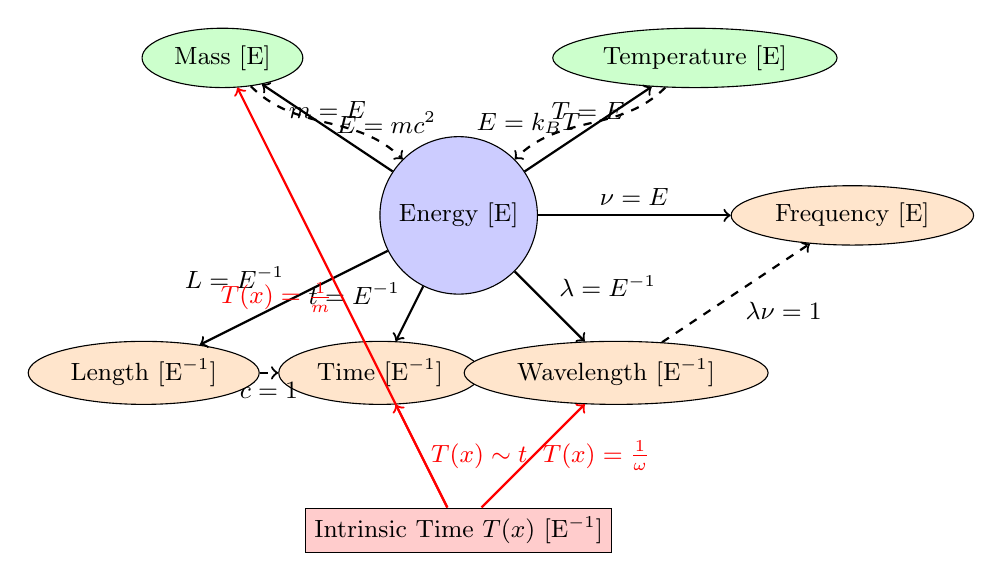
\begin{tikzpicture}
			\small % Smaller font size for the entire diagram
			% Central energy unit
			\node[draw, circle, fill=blue!20, minimum size=2cm] (energy) at (0,0) {Energy [E]};
			
			% Upper branches
			\node[draw, ellipse, fill=green!20] (mass) at (-3,2) {Mass [E]};
			\node[draw, ellipse, fill=green!20] (temp) at (3,2) {Temperature [E]};
			
			% Lower branches
			\node[draw, ellipse, fill=orange!20] (length) at (-4,-2) {Length [E$^{-1}$]};
			\node[draw, ellipse, fill=orange!20] (time) at (-1,-2) {Time [E$^{-1}$]};
			\node[draw, ellipse, fill=orange!20] (wavelength) at (2,-2) {Wavelength [E$^{-1}$]};
			\node[draw, ellipse, fill=orange!20] (frequency) at (5,0) {Frequency [E]};
			
			% Central connection
			\node[draw, rectangle, fill=red!20] (tfield) at (0,-4) {Intrinsic Time $\Tfield$ [E$^{-1}$]};
			
			% Connecting lines
			\draw[->, thick] (energy) -- (mass) node[midway, above] {$m = E$};
			\draw[->, thick] (energy) -- (temp) node[midway, above] {$T = E$};
			\draw[->, thick] (energy) -- (length) node[midway, above left] {$L = E^{-1}$};
			\draw[->, thick] (energy) -- (time) node[midway, above left] {$t = E^{-1}$};
			\draw[->, thick] (energy) -- (wavelength) node[midway, above right] {$\lambda = E^{-1}$};
			\draw[->, thick] (energy) -- (frequency) node[midway, above] {$\nu = E$};
			
			\draw[->, thick, dashed] (length) -- (time) node[midway, below] {$c = 1$};
			\draw[->, thick, dashed] (wavelength) -- (frequency) node[midway, below right] {$\lambda\nu = 1$};
			\draw[->, thick, dashed] (mass) to[out=-45, in=135] node[midway, right] {$E = mc^2$} (energy);
			\draw[->, thick, dashed] (temp) to[out=-135, in=45] node[midway, left] {$E = k_B T$} (energy);
			
			\draw[->, thick, red] (tfield) -- (mass) node[midway, left] {$\Tfield = \frac{1}{m}$};
			\draw[->, thick, red] (tfield) -- (time) node[midway, right] {$\Tfield \sim t$};
			\draw[->, thick, red] (tfield) -- (wavelength) node[midway, right] {$\Tfield = \frac{1}{\omega}$};
		\end{tikzpicture}
		\caption{Network of ratios between physical quantities in the T0 model. All quantities can be traced back to energy [E] as the fundamental unit. Solid lines indicate direct dimensional relationships, dashed lines show physical equivalences through dimensionless constants ($c = k_B = 1$). Red lines represent the mediating role of the intrinsic time field $\Tfield$.}
		\label{fig:quantity_network}
	\end{figure}
	
	\subsection{Quantitative Ratios and Scale Hierarchy}
	
	The quantitative ratios between different scales form a hierarchical structure:
	
	\begin{figure}[ht]
		\centering
		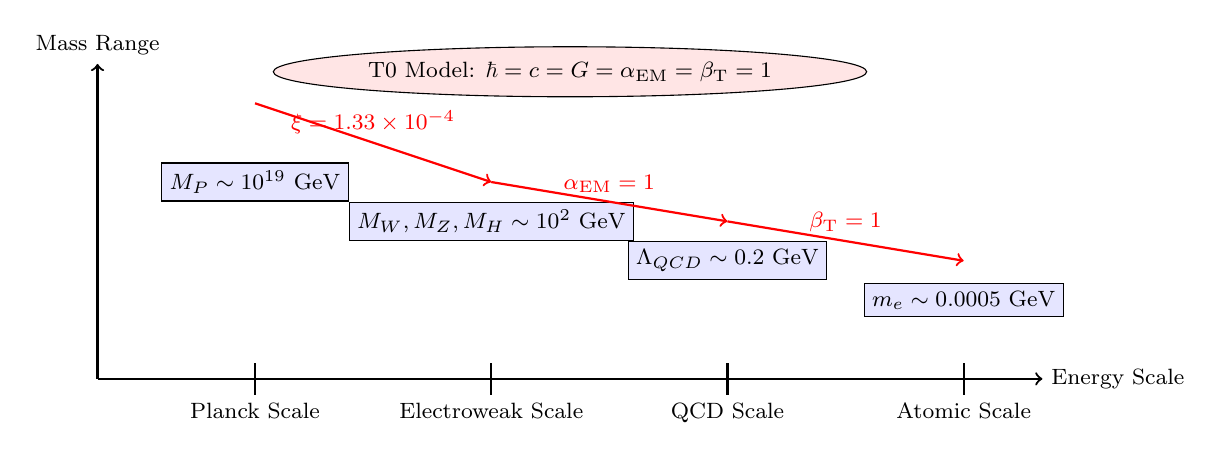
\begin{tikzpicture}
			\footnotesize % Even smaller font size for dense diagram
			% Energy scale axis
			\draw[thick, ->] (0,0) -- (12,0) node[right] {Energy Scale};
			\draw[thick, ->] (0,0) -- (0,4) node[above] {Mass Range};
			
			% Scale markings
			\draw[thick] (2,0.2) -- (2,-0.2) node[below] {Planck Scale};
			\draw[thick] (5,0.2) -- (5,-0.2) node[below] {Electroweak Scale};
			\draw[thick] (8,0.2) -- (8,-0.2) node[below] {QCD Scale};
			\draw[thick] (11,0.2) -- (11,-0.2) node[below] {Atomic Scale};
			
			% Mass/energy markings
			\node[draw, fill=blue!10] at (2,2.5) {$M_P \sim 10^{19}$ GeV};
			\node[draw, fill=blue!10] at (5,2) {$M_W, M_Z, M_H \sim 10^2$ GeV};
			\node[draw, fill=blue!10] at (8,1.5) {$\Lambda_{QCD} \sim 0.2$ GeV};
			\node[draw, fill=blue!10] at (11,1) {$m_e \sim 0.0005$ GeV};
			
			% T0 parameters
			\draw[thick, red, ->] (2,3.5) -- (5,2.5) node[midway, above] {$\xi = 1.33 \times 10^{-4}$};
			\draw[thick, red, ->] (5,2.5) -- (8,2) node[midway, above] {$\alphaEM = 1$};
			\draw[thick, red, ->] (8,2) -- (11,1.5) node[midway, above] {$\betaT = 1$};
			
			% T0 model specifics
			\node[draw, ellipse, fill=red!10] at (6,3.9) {T0 Model: $\hbar = c = G = \alphaEM = \betaT = 1$};
		\end{tikzpicture}
		\caption{Hierarchy of energy scales in the T0 model. The dimensionless constants ($\xi$, $\alphaEM$, $\betaT$) connect the various energy scales from the Planck scale to the atomic scale. In the T0 model with $\hbar = c = G = \alphaEM = \betaT = 1$, these scales are linked by pure numerical ratios, with energy as the fundamental unit.}
		\label{fig:energy_hierarchy}
	\end{figure}
	
	\subsection{Ratios of Fundamental Forces in Natural Units}
	
	In the T0 model with a unified natural unit system, the fundamental interactions can be characterized by their dimensionless coupling constants:
	
	\begin{table}[ht]
		\centering
		\begin{adjustbox}{scale=0.95}
			\begin{tabular}{llll}
				\hline
				\textbf{Force} & \textbf{Dimensionless Coupling} & \textbf{Natural Value} & \textbf{Range} \\
				\hline
				Electromagnetic & $\alphaEM$ & 1 & $\infty$ \\
				Strong & $\alpha_s$ & $\sim 0.118$ at $Q^2=M_Z^2$ & $\sim 10^{-15}$ m \\
				Weak & $\alpha_W = g^2/(4\pi)$ & $\sim 1/30$ & $\sim 10^{-18}$ m \\
				Gravitation & $\alpha_G = Gm^2/\hbar c$ & $m^2/m_P^2$ & $\infty$ \\
				\hline
				\multicolumn{3}{c}{} \\
				\hline
			\end{tabular}
		\end{adjustbox}
		\caption{Fundamental Forces in Natural Units}
		\label{tab:forces}
	\end{table}
	
	In the T0 model, these ratios are reinterpreted: Gravitation is no longer a fundamental force but an emergent property of the intrinsic time field $\Tfield$, leading to a natural unification \cite{pascher_grundkraefte_2025}.
	
	\section{Role of Energy as the Fundamental Unit}
	
	In the unified natural unit system of the T0 model, energy [E] serves as the fundamental unit from which all other physical quantities can be derived:
	
	\subsection{Practical Notations in Natural Units}
	
	\begin{table}[ht]
		\centering
		\begin{adjustbox}{scale=1.2}
			\begin{tabular}{lll}
				\hline
				\textbf{Physical Quantity} & \textbf{Natural Unit} & \textbf{Practical Notation} \\
				\hline
				Length & [E$^{-1}$] & eV$^{-1}$, GeV$^{-1}$, TeV$^{-1}$ \\
				Time & [E$^{-1}$] & eV$^{-1}$, GeV$^{-1}$, TeV$^{-1}$ \\
				Mass/Energy & [E] & eV, MeV, GeV, TeV \\
				Temperature & [E] & eV, MeV \\
				Momentum & [E] & eV, GeV \\
				Cross Section & [E$^{-2}$] & GeV$^{-2}$, mb, pb, fb \\
				Decay Rate & [E] & eV, MeV \\
				\hline
				\multicolumn{2}{c}{} \\
				\hline
			\end{tabular}
		\end{adjustbox}
		\caption{Practical Notations of Physical Quantities in Natural Units}
		\label{tab:practical_notation}
	\end{table}
	
	\begin{figure}[ht]
		\centering
		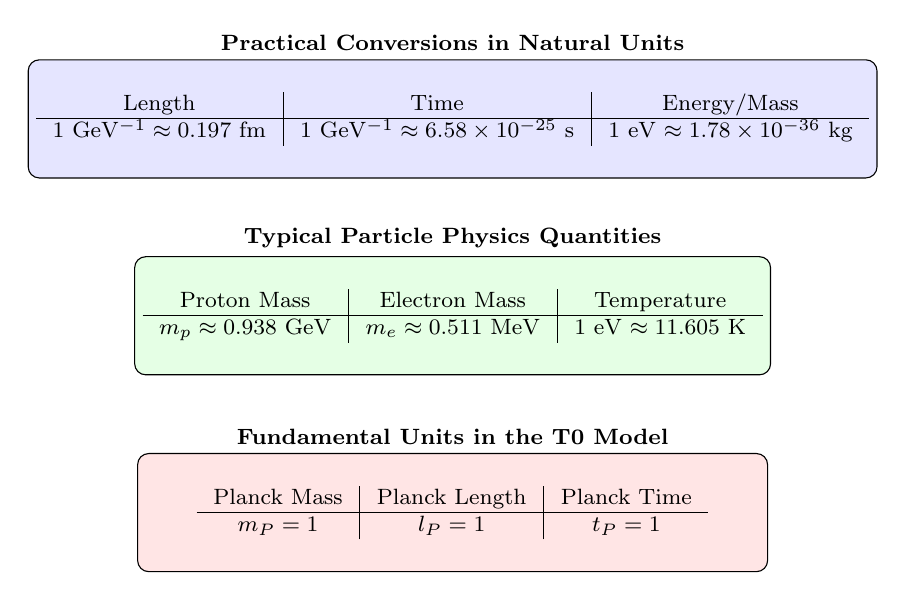
\begin{tikzpicture}
			\footnotesize % Smaller font size for the diagram
			% Conversion schema
			\node[draw, rounded corners, fill=blue!10, minimum width=8cm, minimum height=1.5cm] (conversion) at (0,0) {
				\begin{tabular}{c|c|c}
					Length & Time & Energy/Mass \\
					\hline
					1 GeV$^{-1} \approx 0.197$ fm & 1 GeV$^{-1} \approx 6.58 \times 10^{-25}$ s & 1 eV $\approx 1.78 \times 10^{-36}$ kg
				\end{tabular}
			};
			
			\node[draw, rounded corners, fill=green!10, minimum width=8cm, minimum height=1.5cm] (practical) at (0,-2.5) {
				\begin{tabular}{c|c|c}
					Proton Mass & Electron Mass & Temperature \\
					\hline
					$m_p \approx 0.938$ GeV & $m_e \approx 0.511$ MeV & 1 eV $\approx 11.605$ K
				\end{tabular}
			};
			
			\node[draw, rounded corners, fill=red!10, minimum width=8cm, minimum height=1.5cm] (fundamental) at (0,-5) {
				\begin{tabular}{c|c|c}
					Planck Mass & Planck Length & Planck Time \\
					\hline
					$m_P = 1$ & $l_P = 1$ & $t_P = 1$
				\end{tabular}
			};
			
			\node[above] at (conversion.north) {\textbf{Practical Conversions in Natural Units}};
			\node[above] at (practical.north) {\textbf{Typical Particle Physics Quantities}};
			\node[above] at (fundamental.north) {\textbf{Fundamental Units in the T0 Model}};
		\end{tikzpicture}
		\caption{Practical conversions between SI units and natural units, as well as typical quantities in particle physics. In the T0 model with $\hbar = c = G = \alphaEM = \betaT = 1$, all Planck units are normalized to 1, and all physical quantities can be expressed in multiples or fractions of these units.}
		\label{fig:practical_conversion}
	\end{figure}
	
	\subsection{Philosophical Implications}
	
	The use of energy as the fundamental unit in the T0 model has profound philosophical implications:
	
	\begin{enumerate}
		\item \textbf{Ontological Simplification:} Energy becomes the fundamental entity from which all other physical quantities can be derived. This aligns with Einstein’s equivalence of mass and energy and extends it to all physical quantities.
		
		\item \textbf{Unified Description of Nature:} The use of natural units with $\hbar = c = G = \alphaEM = \betaT = 1$ enables a unified description of all known physical phenomena without arbitrary dimensioned constants.
		
		\item \textbf{Emergent Space-Time:} In the T0 model, space-time can be considered an emergent phenomenon arising from the properties of the intrinsic time field $\Tfield$. This corresponds to modern approaches in theoretical physics that view space and time as emergent properties of a more fundamental substrate \cite{pascher_perspective_2025, pascher_zeit_2025}.
		
		\item \textbf{Overcoming the Mind-Body Problem:} The introduction of absolute time in the T0 model, alongside the reinterpretation of relativistic effects as mass variation, offers a new approach to understanding consciousness and its relationship to the physical world \cite{pascher_perspective_2025}.
	\end{enumerate}
	
	The unification through energy as the fundamental unit is not just a mathematical simplification but reflects the intrinsic unity of natural laws as postulated in the T0 model \cite{pascher_dualismus_2025}.
	
	\section{Summary and Outlook}
	
	The unified natural unit system of the T0 model with $\hbar = c = G = k_B = \alphaEM = \alpha_W = \betaT = 1$ provides an elegant framework for unifying all physical phenomena with energy as the fundamental unit. The key findings are:
	
	\begin{enumerate}
		\item \textbf{Hierarchical Structure:} Physical constants and scales form a clear hierarchical structure, with all quantities reducible to energy [E] as the fundamental unit.
		
		\item \textbf{Simplified Field Equations:} The fundamental equations of physics take particularly elegant forms in this system, revealing the intrinsic unity of natural laws.
		
		\item \textbf{Bridge Between Quantum Mechanics and Relativity:} The intrinsic time field $\Tfield$ serves as a mediator between quantum mechanics and relativity, bridging micro- and macro-scales.
		
		\item \textbf{Emergent Gravitation:} Gravitation is reinterpreted as an emergent phenomenon from the intrinsic time field $\Tfield$, without assuming a fundamental gravitational interaction.
		
		\item \textbf{Natural Explanation of Cosmological Phenomena:} The T0 model offers natural explanations for phenomena such as redshift, cosmic expansion, and dark energy, without requiring ad-hoc assumptions like inflation or dark matter.
	\end{enumerate}
	
	Future research directions could include:
	
	\begin{itemize}
		\item \textbf{Experimental Tests of Wavelength-Dependent Redshift:} $z(\lambda) = z_0(1+\ln(\lambda/\lambda_0))$, which would enable a direct test of the parameter $\betaT = 1$.
		
		\item \textbf{Precision Measurements of Atomic Energy Levels:} The reinterpretation of the Rydberg constant as $R_\infty = 1/2$ in natural units could lead to new experimental tests.
		
		\item \textbf{Quantum Field Theoretical Development of the T0 Model:} The complete quantization of the intrinsic time field $\Tfield$ and its embedding in a quantum field theoretical framework remains a significant challenge.
		
		\item \textbf{Numerical Simulations of Cosmological Evolution:} Using the modified gravitational potential $\Phi(r) = -\frac{M}{r} + r$, computer simulations of galaxy dynamics could be conducted to compare T0 model predictions with astronomical observations.
	\end{itemize}
	
	The unified natural unit system of the T0 model with energy as the fundamental unit offers a promising approach to overcoming the divide between quantum mechanics and relativity and could lead to a deeper understanding of the fundamental structure of the universe \cite{pascher_vereinheitlichung_2025}.
	
	\bibliographystyle{apsrev4-2}
	\begin{thebibliography}{99}
		\bibitem{pascher_zeit_2025} J. Pascher, \href{https://github.com/jpascher/T0-Time-Mass-Duality/tree/main/2/pdf/English/ZeitEmergentQMEn.pdf}{Time as an Emergent Property in Quantum Mechanics: A Connection Between Relativity, Fine-Structure Constant, and Quantum Dynamics}, March 23, 2025.
		\bibitem{pascher_messdifferenzen_2025} J. Pascher, \href{https://github.com/jpascher/T0-Time-Mass-Duality/tree/main/2/pdf/English/MessdifferenzenT0StandardEn.pdf}{Compensatory and Additive Effects: An Analysis of Measurement Differences Between the T0 Model and the $\Lambda$CDM Standard Model}, April 2, 2025.
		\bibitem{pascher_galaxies_2025} J. Pascher, \href{https://github.com/jpascher/T0-Time-Mass-Duality/tree/main/2/pdf/English/MassVarGalaxienEn.pdf}{Mass Variation in Galaxies: An Analysis in the T0 Model with Emergent Gravitation}, March 30, 2025.
		\bibitem{pascher_params_2025} J. Pascher, \href{https://github.com/jpascher/T0-Time-Mass-Duality/tree/main/2/pdf/English/ZeitMasseT0ParamsEn.pdf}{Time-Mass Duality Theory (T0 Model): Derivation of Parameters $\kappa$, $\alpha$, and $\beta$}, March 30, 2025.
		\bibitem{pascher_temp_2025} J. Pascher, \href{https://github.com/jpascher/T0-Time-Mass-Duality/tree/main/2/pdf/English/NatEinheitenAlpha1En.pdf}{Adjustment of Temperature Units in Natural Units and CMB Measurements}, April 2, 2025.
		\bibitem{pascher_alpha_2025} J. Pascher, \href{https://github.com/jpascher/T0-Time-Mass-Duality/tree/main/2/pdf/English/NatEinheitenAlpha1En.pdf}{Energy as a Fundamental Unit: Natural Units with $\alphaEM = 1$ in the T0 Model}, March 26, 2025.
		\bibitem{pascher_beta_2025} J. Pascher, \href{https://github.com/jpascher/T0-Time-Mass-Duality/tree/main/2/pdf/English/Alpha1Beta1KonsistenzEn.pdf}{Dimensionless Parameters in the T0 Model: Setting $\beta = 1$ in Natural Units}, April 4, 2025.
		\bibitem{pascher_higgs_2025} J. Pascher, \href{https://github.com/jpascher/T0-Time-Mass-Duality/tree/main/2/pdf/English/MathHiggsZeitMasseEn.pdf}{Mathematical Formulation of the Higgs Mechanism in Time-Mass Duality}, March 28, 2025.
		\bibitem{pascher_lagrange_2025} J. Pascher, \href{https://github.com/jpascher/T0-Time-Mass-Duality/tree/main/2/pdf/English/MathZeitMasseLagrangeEn.pdf}{From Time Dilation to Mass Variation: Mathematical Core Formulations of Time-Mass Duality Theory}, March 29, 2025.
		\bibitem{pascher_emergente_2025} J. Pascher, \href{https://github.com/jpascher/T0-Time-Mass-Duality/tree/main/2/pdf/English/EmergentGravT0En.pdf}{Emergent Gravitation in the T0 Model: A Comprehensive Derivation}, April 1, 2025.
		\bibitem{pascher_perspective_2025} J. Pascher, \href{https://github.com/jpascher/T0-Time-Mass-Duality/tree/main/2/pdf/English/ZeitRaumPascherEn.pdf}{A New Perspective on Time and Space: Johann Pascher's Revolutionary Ideas}, March 25, 2025.
		\bibitem{pascher_dualismus_2025} J. Pascher, \href{https://github.com/jpascher/T0-Time-Mass-Duality/tree/main/2/pdf/English/KurzKomplementDualPhysikEn.pdf}{In Brief - Complementary Duality in Physics: From Wave-Particle to Time-Mass Concept}, March 26, 2025.
		\bibitem{pascher_grundkraefte_2025} J. Pascher, \href{https://github.com/jpascher/T0-Time-Mass-Duality/tree/main/2/pdf/English/VierKraefteZeitMasseEn.pdf}{Simplified Description of the Fundamental Forces with Time-Mass Duality}, March 27, 2025.
		\bibitem{pascher_zeit_masse_2025} J. Pascher, \href{https://github.com/jpascher/T0-Time-Mass-Duality/tree/main/2/pdf/English/ZeitMasseNeuerBlickEn.pdf}{Time and Mass: A New Look at Old Formulas – and Liberation from Traditional Constraints}, March 22, 2025.
		\bibitem{pascher_quantum_2025} J. Pascher, \href{https://github.com/jpascher/T0-Time-Mass-Duality/tree/main/2/pdf/English/NotwendigkeitQMErweiterungEn.pdf}{The Necessity of Extending Standard Quantum Mechanics and Quantum Field Theory}, March 27, 2025.
		\bibitem{pascher_photons_2025} J. Pascher, \href{https://github.com/jpascher/T0-Time-Mass-Duality/tree/main/2/pdf/English/DynMassePhotonenNichtlokalEn.pdf}{Dynamic Mass of Photons and Its Implications for Nonlocality in the T0 Model}, March 25, 2025.
		\bibitem{pascher_alphabeta_2025} J. Pascher, \href{https://github.com/jpascher/T0-Time-Mass-Duality/tree/main/2/pdf/English/Alpha1Beta1KonsistenzEn.pdf}{Unified Unit System in the T0 Model: The Consistency of $\alpha = 1$ and $\beta = 1$}, April 5, 2025.
		\bibitem{pascher_planck_2025} J. Pascher, \href{https://github.com/jpascher/T0-Time-Mass-Duality/tree/main/2/pdf/English/JenseitsPlanckEn.pdf}{Real Consequences of Reformulating Time and Mass in Physics: Beyond the Planck Scale}, March 24, 2025.
		\bibitem{pascher_energiedynamik_2025} J. Pascher, \href{https://github.com/jpascher/T0-Time-Mass-Duality/tree/main/2/pdf/English/MathEnergiedynamikEn.pdf}{Dark Energy in the T0 Model: A Mathematical Analysis of Energy Dynamics}, April 3, 2025.
		\bibitem{pascher_vereinheitlichung_2025} J. Pascher, \href{https://github.com/jpascher/T0-Time-Mass-Duality/tree/main/2/pdf/English/T0VereinheitlichungDEGalEn.pdf}{Unification of the T0 Model: Foundations, Dark Energy, and Galaxy Dynamics}, April 4, 2025.
		\bibitem{pascher_formalismen_2025} J. Pascher, \href{https://github.com/jpascher/T0-Time-Mass-Duality/tree/main/2/pdf/English/MathZeitMasseLagrangeEn.pdf}{From Time Dilation to Mass Variation: Mathematical Core Formulations of Time-Mass Duality Theory}, April 5, 2025.
		\bibitem{Planck1899} M. Planck, \textit{On Irreversible Radiation Processes}, Proceedings of the Royal Prussian Academy of Sciences in Berlin 5, 440-480 (1899).
		\bibitem{Dirac1928} P. A. M. Dirac, \textit{The Quantum Theory of the Electron}, Proceedings of the Royal Society of London A 117, 610-624 (1928).
		\bibitem{Einstein1905} A. Einstein, \textit{On the Electrodynamics of Moving Bodies}, Annalen der Physik 322, 891-921 (1905).
		\bibitem{Einstein1915} A. Einstein, \textit{The Field Equations of Gravitation}, Proceedings of the Royal Prussian Academy of Sciences, 844-847 (1915).
		\bibitem{Sommerfeld1916} A. Sommerfeld, \textit{On the Quantum Theory of Spectral Lines}, Annalen der Physik 356, 1-94 (1916).
		\bibitem{Heisenberg1927} W. Heisenberg, \textit{On the Perceptual Content of Quantum Theoretical Kinematics and Mechanics}, Zeitschrift für Physik 43, 172-198 (1927).
		\bibitem{Schrodinger1926} E. Schrödinger, \textit{Quantization as an Eigenvalue Problem}, Annalen der Physik 384, 361-376 (1926).
		\bibitem{Feynman1985} R. P. Feynman, \textit{QED: The Strange Theory of Light and Matter}, Princeton University Press (1985).
		\bibitem{Duff2002} M. J. Duff, L. B. Okun \& G. Veneziano, \textit{Trialogue on the Number of Fundamental Constants}, Journal of High Energy Physics 3, 023 (2002).
		\bibitem{Wilczek2008} F. Wilczek, \textit{The Lightness of Being: Mass, Ether, and the Unification of Forces}, Basic Books (2008).
		\bibitem{Verlinde2011} E. Verlinde, \textit{On the Origin of Gravity and the Laws of Newton}, Journal of High Energy Physics 4, 29 (2011).
		\bibitem{Greene2020} B. Greene, \textit{Until the End of Time: Mind, Matter, and Our Search for Meaning in an Evolving Universe}, Alfred A. Knopf (2020).
		\bibitem{tHooft1993} G. 't Hooft, \textit{Dimensional Reduction in Quantum Gravity}, arXiv:gr-qc/9310026 (1993).
		\bibitem{Will2014} C. M. Will, \textit{The Confrontation between General Relativity and Experiment}, Living Reviews in Relativity 17, 4 (2014).
	\end{thebibliography}
	
\end{document}